\section{EFX Orientations}

The following observations will be useful throughout this section. Recall the definition of \emph{strong} envy from \cref{def:envy}.

\begin{observation}\label{obs:EFX_one_good}
    An agent that has only received one good is not strongly envied by any agent.
\end{observation}

\begin{observation}\label{obs:EFX_zero_value}
    For agents $i,j$, if $i$ does not strongly envy~$j$ and $j$ has received a good $g$ s.t.~$v_i(g) = 0$, then $i$ does not envy $j$.
\end{observation}

\subsection{From EF to EFX Orientations}\label{subsec:EF->EFX}


It was first proven by Christodoulou et al.~\cite{EFXgraphs} that \EFXo\ is NP-complete even with symmetric valuations;
this hardness persists even for simple graphs of vertex cover number $8$ or for multigraphs consisting of $10$ vertices,
where the problem was proven to be weakly NP-complete (Deligkas et al.~\cite{ijcai/DeligkasEGK25}).
In a follow-up work, Afshinmehr et al.~\cite{AfshinmehrDKMR25} show NP-completeness even for symmetric instances on bipartite multigraphs with $8$ vertices.
Here we present a reduction from \EFo\ to \EFXo\ that, along with \cref{subsec:EF:hardness},
will allow us to complement and improve upon the aforementioned results. See \cref{fig:EF_to_EFX_main} for an overview of our reduction.


   \begin{figure}[ht]
        \centering
        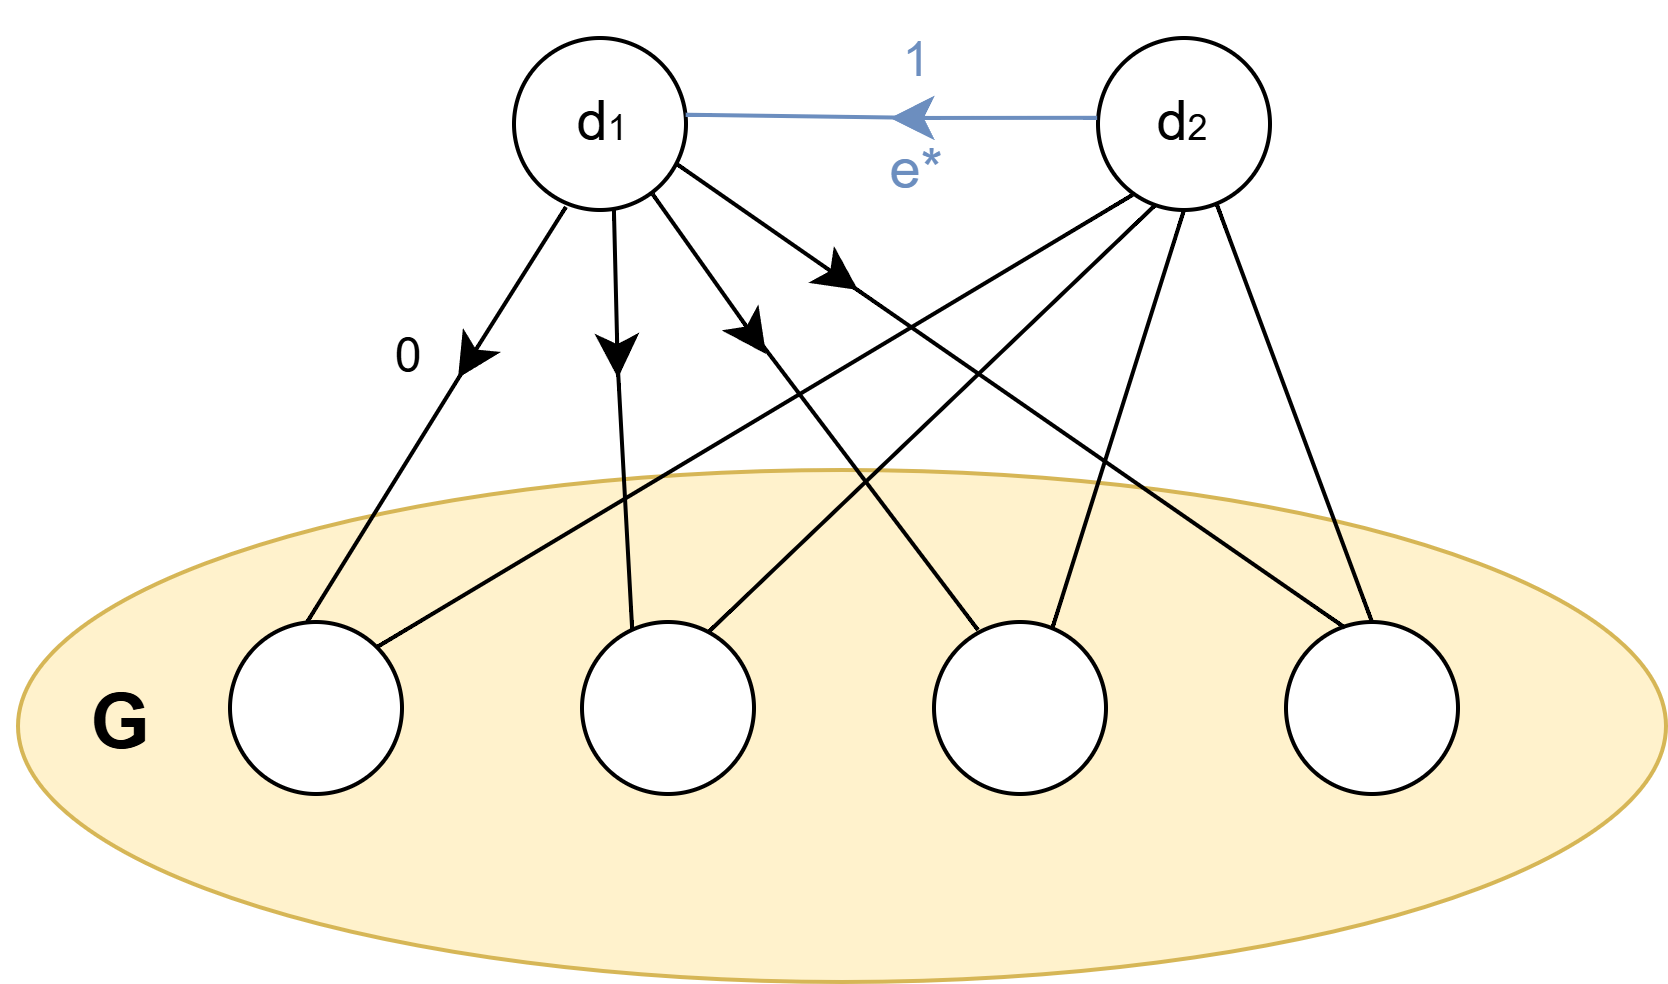
\includegraphics[width=0.5\linewidth]{Images/reduction.png}
        \caption{Our reduction from \EFo\ to \EFXo\ in \cref{thm:efo->efxo}. If $e^*$ is oriented towards~$d_1$, then all other edges incident to $d_1$ must be oriented away from $d_1$ to obtain an EFX orientation. Every $v\in G$ receives an edge of weight $0$, which forces equivalence between EF and EFX by \cref{obs:EFX_zero_value}. A symmetrical argument holds if $e^*$ is oriented towards $d_2$. For more details, see Appendix C.}
        \label{fig:EF_to_EFX_main}
    \end{figure}

\begin{theoremrep}[\appsymb]\label{thm:efo->efxo}
    There is a polynomial-time, logarithmic-space reduction from \EFo\ to \EFXo\ that only adds 2 vertices
    and edges of symmetric binary valuation.
    The reduction preserves simplicity.
\end{theoremrep}

\begin{proof}
    Let $\mathcal{I}=(G=(V,E),\{v_i\}_{i\in V})$ be an instance of \EFo.
    We build an $\EFXo$ instance $\mathcal{I'}$ by adding two vertices $d_1,d_2$ to $G$, each connected with every $v\in V$ by edges of weight $0$ (for both endpoints). Additionally, we connect $d_1$ and $d_2$ with an edge $e^*$ of weight $1$ (for both endpoints). Let $G'=(V',E')$ be the resulting graph of~$\mathcal{I}'$ (see \cref{fig:EF_to_EFX}).

    \begin{figure}[ht]
        \centering
        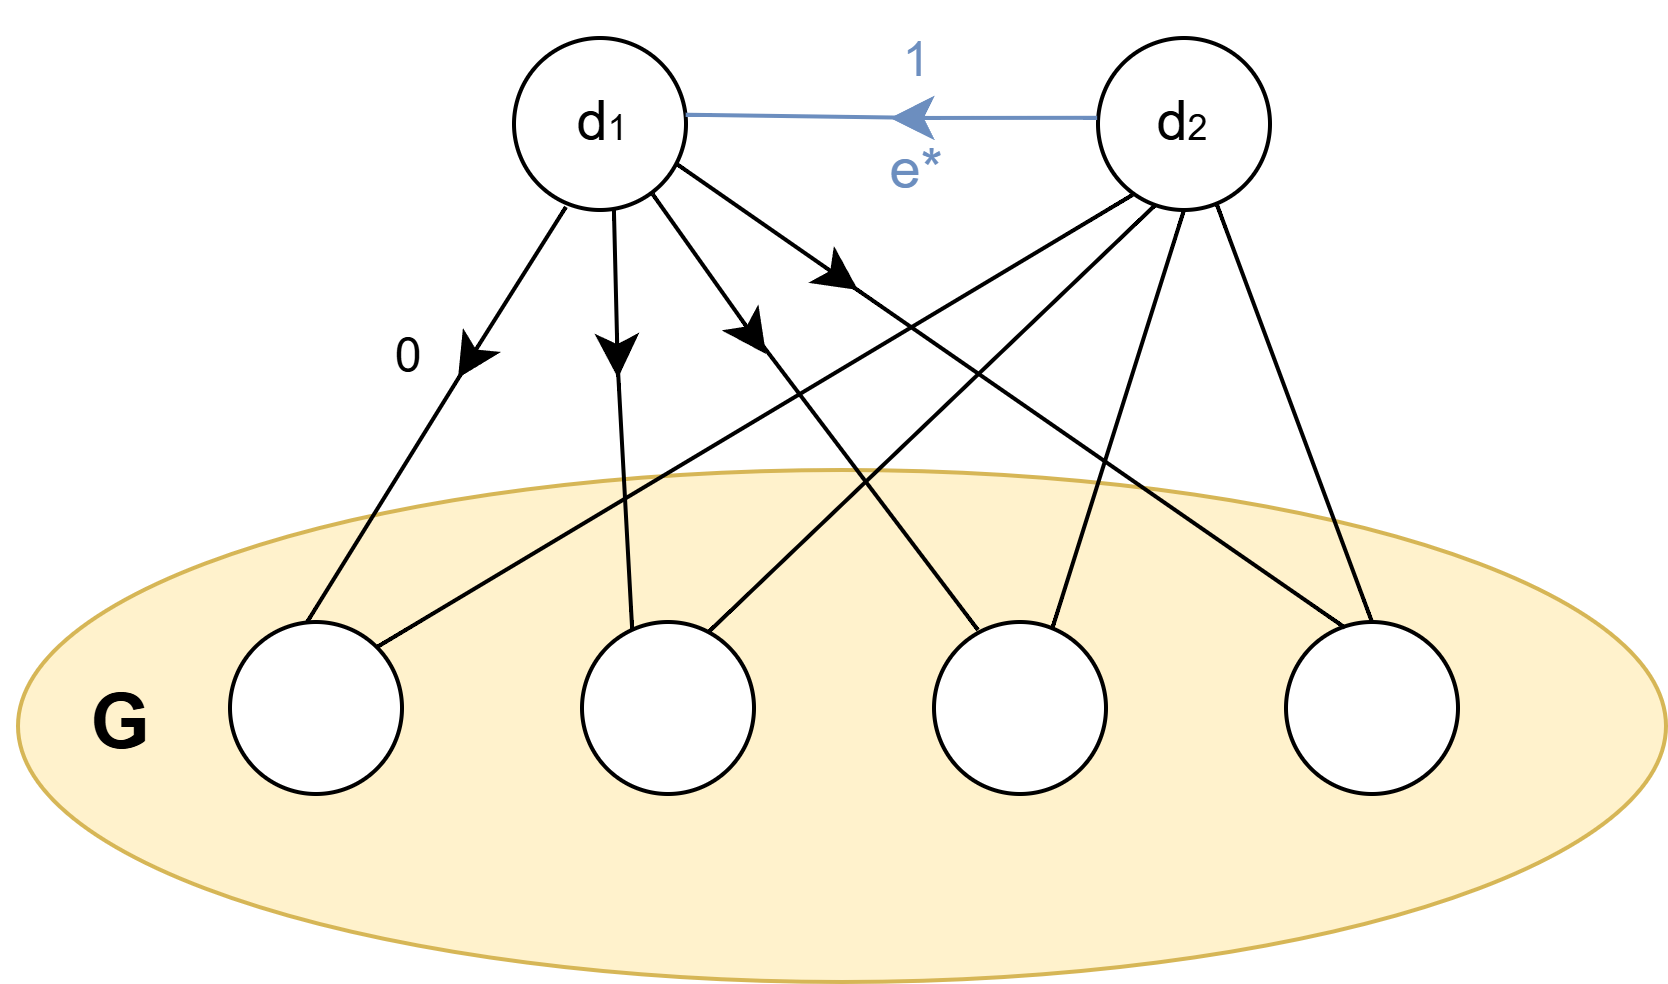
\includegraphics[width=0.5\linewidth]{Images/reduction.png}
        \caption{Our reduction from \EFo\ to \EFXo. If $e^*$ is oriented towards~$d_1$, then all other edges incident to $d_1$ must be oriented away from $d_1$ to obtain an EFX orientation. Every $v\in G$ receives an edge of weight $0$, which forces equivalence between EF and EFX by \cref{obs:EFX_zero_value}. A symmetrical argument holds if $e^*$ is oriented towards $d_2$.}
        \label{fig:EF_to_EFX}
    \end{figure}

    We prove that if $\mathcal{I}$ has an EF orientation, then $\mathcal{I}'$ has an EFX orientation. Take an EF orientation $O$ of $\mathcal{I}$ and extend it by orienting the edges in $E'\setminus E$ as follows to obtain an orientation~$O'$.
    Orient $e^*$ towards $d_1$. Then, orient all other edges incident to $d_2$ towards $d_2$ and all other edges incident to $d_1$ away from $d_1$. By \cref{obs:EFX_one_good}, $d_1$ is not strongly envied by any $v\in V'$; the same holds for $d_2$ since all of its allocated edges are of weight $0$ (for both endpoints). Additionally, $d_1$ does not envy any other vertex, since
    it has received its unique incident edge with non-zero weight. Observe that $d_2$ only envies $d_1$, since it has received all of its incident edges except $e^*$ (however, this envy is not strong, by \cref{obs:EFX_one_good}). Since $O$ is EF, it holds that $u$ does not envy $v$ for all $u,v \in V$, implying that $u$ does not strongly envy $v$. From all the above we infer that $O'$ is EFX.

    We now prove the converse: if $\mathcal{I}'$ has an EFX orientation, then $\mathcal{I}$ has an EF orientation. Take an EFX orientation $O'$ of $\mathcal{I}'$. Without loss of generality, assume $e^*$ is oriented towards $d_1$ in $O'$. Then, for $O'$ to be an EFX orientation, $d_1$ must not receive any other edge (otherwise $d_2$ would strongly envy $d_1$), implying that all other edges incident to $d_1$ are oriented away from $d_1$ in $O'$. Hence, every vertex $v\in V$ has received a zero-weight edge in $O'$. For all $u,v\in V$, $u$ does not strongly envy $v$ because $O'$ is EFX; by \cref{obs:EFX_zero_value}, this implies that $u$ does not envy $v$. Hence, orienting all edges in $E$ in accordance to $O'$ results in an EF orientation $O$ of $\mathcal{I}$.

    The reduction described uses logarithmic space,%
    \footnote{This property is essential for the XNLP- and XALP-hardness in \cref{cor:EFXo_W1}.}
    since only two vertices and $\bO(n)$ edges of polynomial weight are added to the graph.
\end{proof}

Combining \cref{thm:efo->efxo} with the hardness results in \cref{subsec:EF:hardness} leads to \cref{cor:EFXo:weak_NPh,cor:EFXo_W1}.

\begin{corollary}\label{cor:EFXo:weak_NPh}
    {\EFXo} is weakly NP-complete even restricted to
    \begin{itemize}
        \item simple symmetric instances of vertex cover number $4$,
        \item symmetric instances with $4$ vertices.
    \end{itemize}
\end{corollary}

\begin{corollary}\label{cor:EFXo_W1}
    \EFXo\ is  W[1]-hard parameterized by vertex cover number,
    XNLP-hard parameterized by pathwidth,
    and XALP-hard parameterized by treewidth,
    even restricted to simple symmetric instances with polynomially-bounded weights.
    Furthermore, for such instances, {\EFXo} does not admit a $n^{o(\vc)}$ algorithm under the ETH,
    where $\vc$ denotes the vertex cover number of the input graph.
\end{corollary}

We now compare \cref{cor:EFXo:weak_NPh,cor:EFXo_W1} with existing literature.
\cref{cor:EFXo:weak_NPh} improves upon the respective constants of 8 and 10 from Deligkas et al.~\cite{ijcai/DeligkasEGK25}, as well as the result for multigraphs with~8 vertices by Afshinmehr et al.~\cite{AfshinmehrDKMR25}.
As for \cref{cor:EFXo_W1}, it presents the first hardness results for instances with polynomially-bounded weights and small vertex cover,
and along with the algorithm of \cref{subsec:EFXo:tw}, it answers an open question of Deligkas et al.~\cite{ijcai/DeligkasEGK25} regarding the hardness of {\EFXo} in this setting.

% we complement this lower bound with the algorithm of \cref{thm:EFX:tw}.


% \begin{corollary}\label{cor:EFXo_XALP_XNLP}
%     \EFXo\ is $XNLP$-hard parameterized by pathwidth and $XALP$-hard parameterized by treewidth, even restricted to
%     \begin{itemize}
%         \item simple symmetric instances with polynomially-bounded values,
%         \item symmetric instances with values at most $3$,
%         \item instances with values at most $2$.
%     \end{itemize}
% \end{corollary}

\subsection{Parameterization by Treewidth plus Maximum Shared Weight}\label{subsec:EFXo:tw}

Moving on, we consider the {\EFXo} problem on graphs of small treewidth.
As previously mentioned, if one allows binary-encoded weights, then the problem remains
NP-hard even for simple graphs of constant vertex cover, or multigraphs with constant number
of vertices. Consequently, in the following we consider the case where all weights are polynomially-bounded;
this is exactly the regime for which Deligkas et al.~\cite{ijcai/DeligkasEGK25} have explicitly asked whether
the structure of the input graph may prove algorithmically useful.
For this case, \cref{cor:EFXo_W1} already gives a $n^{o(\vc)}$ lower bound under the ETH even on
simple graphs. Our main contribution in this section is to complement this lower bound with a DP algorithm parameterized by treewidth
plus maximum shared weight, in a similar fashion as in \cref{thm:ef:fpt_tw};
for polynomially-bounded weights where $W = (n+m)^{\bO(1)}$ this results in an algorithm of running time $(n+m)^{\bO(\tw)}$.
Again, our algorithm works even for the more general {\EFXmc} problem, and for multigraphs with non-identical valuations.

We first state the following observation.

\begin{observation}\label{obs:efx_zero_value_goods}
    Let an instance of {\EFXo} where vertices~$i,j$ share more than one edges of weight~$0$ for both endpoints.
    Then, removing all but one of those edges results in an equivalent instance.
\end{observation}

To see why \cref{obs:efx_zero_value_goods} holds, notice that any EFX orientation that does not orient all such edges to a \emph{single} endpoint,
can be modified to an EFX orientation that does.

\begin{theoremrep}[\appsymb]\label{thm:EFX:tw}
    Given an instance $\mathcal{I}$ of \EFXmc\ along with a nice tree decomposition of the input multigraph of width $\tw$,
    one can decide $\mathcal{I}$ in time $W^{\bO(\tw)} (n + m)^{\bO(1)}$,
    where $W$ denotes the maximum shared weight of $\mathcal{I}$ and $n$ the number of agents.
\end{theoremrep}

% FOR ARXIV, PROOF IS IN COMMENTS @EDOUARD

% \begin{proof}
%     The proof is analogous to the proof of \cref{thm:ef:fpt_tw}, albeit more complicated. We will include it in a revised version of this paper.
% \end{proof}

\begin{proof}
    Let $\mathcal{I} = (G,\{v_i\}_{i\in V})$ denote the instance of {\EFmc}
    and $(T,\{B_t\}_{t\in V(T)})$ the given nice tree decomposition of $G$ of width $\tw$.

    We will use \cref{obs:efx_zero_value_goods} as well as the following one for the correctness of our algorithm:

    \begin{observation}\label{obs:only_one_envious}
        Let $O$ be an orientation.
        If vertex $i$ envies, but not strongly envies, vertex $j$, then
        all edges oriented towards $j$ in $O$ are in $E_{ij}$. This additionally implies that no vertex $v\neq i$ envies $j$ in $O$.
    \end{observation}

    \textbf{Notations and Definitions.}
    Before describing our algorithm we first fix some notations. For $t\in V(T)$, we define $V_t$, $E_t$, $G_t$ and $A_t$ in the same way as in the proof of \cref{thm:ef:fpt_tw}.

    We define $A_t^{ef}$ to be the set of all partial orientations of $G_t$ where, first, all vertices of $V_t$ are  non strongly envious, and second, all vertices of $B_t$ which are envied (but not strongly) by some vertex of $V_t$, are also non strongly envious. Intuitively, those are the partial orientations of $G_t$ that can be completed into an envy-free orientation up to any good of $G$.

    \textbf{Signature definition.} Let $O\in A_t$. We define the \emph{signature} of $O$ with respect to $t$ as a triple $\sigma=(r,d,k)$ with $r\colon B_t\to [0,W]\cup\{None\}$, $d\colon B_t\to [0,W]\cup\{Some\}$ and $k\in [0,|E|]$ defined by:
    \begin{itemize}
        \item for all $i\in B_t$, $r(i)=\begin{cases}
            None & if\ X_i=\varnothing \\
            \min\{v_i(X_i),W\} & otherwise \\
        \end{cases}$

        \item for all $i\in B_t$, $d(i)=\begin{cases}
            Some & if\ there\ is\ \ell\in V_t\ envious\ of\ i\\
            \max_{\ell\in V_t,\ e\in X_\ell}\{v_i(X_\ell\setminus\{e\})\} & otherwise \\
        \end{cases}$

        \item $k=|E_t|-\Sigma_{i\in B_t\cup V_t}|X_i|$
    \end{itemize}

    Let $\Sigma_t$ denote the set of all possible signatures for node $t$, and notice that $|\Sigma_t|\leq |E|(W+2)^{2(tw+1)}$. We define the $\emph{signature function}$ $\sgn_t\colon A_t\to \Sigma_t$ that attributes to each partial orientation of $G_t$ its signature with respect to $t$.

    Take $O\in A_t^{ef}$. As in the algorithm of \cref{thm:ef:fpt_tw}, $sgn_t(O)=(r,d,k)$ has two types of information: $r$ and $d$ are the minimum amount of information needed to complete $O$ into a partial envy-free orientation up to any good: $r(i)$ represents what $i$ already \emph{received} from $O$ up to any good, and if $r(i)=None$, it means that $i$ did not receive any edge yet, and therefore from \cref{obs:EFX_one_good}, it means that in an extension of $O$, one vertex of $V\setminus V_t$ can be envious of $i$ without being strongly envious (note that we can have $r(i)=0$, as edges can have a value of $0$). $d(i)$ represents the amount that $i$ needs to receive to not be strongly envious of the vertices of $V_t$, and if $d(i)=Some$, it means that some vertex $\ell\in V_t$ is envious of $i$ (but not strongly envious), and therefore $i$ cannot receive any other edge, as otherwise $\ell$ would become strongly envious of $i$.

    In the following, we will allow ourselves to use the value $r(i)$ in additions and inequalities, even if it is possible that $r(i)=None$. In that case, we consider that $None$ has value $0$.

    \textbf{Signature valuation definition.} We define the \emph{valuation function} $val_t\colon \Sigma_t\to \{0,1\}$ defined by: for all $\sigma\in \Sigma_t$, $val_t(\sigma)=1$ if and only if there is $O\in A_t^{ef}$ such that $\sgn_t(O)=\sigma$.

    Take $t$ to be the root of $T$; by definition of a nice tree decomposition, $B_t$ is an empty set, $V_t=V$, $E_t=E$ and $G_t=G$. Therefore, $A_t^{ef}$ is exactly the set of all partial envy-free up to any good orientations of $G$. So, if we have an efficient way to compute the values of $val_t$, we can efficiently solve \EFXmc. We present an algorithm that computes the values of $val_t$ for all $t\in V(T)$ dynamically over the nice tree decomposition.

    \textbf{In the following, we describe the algorithm.}

    Take $t\in V(T)$:

    \textbf{Leaf node.} If $t$ is a leaf node, then $B_t=\varnothing$, $V_t=\varnothing$ and $E_t=\varnothing$. Therefore, $A_t=A_t^{ef}=\{\varnothing\}$. Take $epy$ the only function from $\varnothing$ to $[0,W]$, $val_t((epy,epy,0))=1$ and for all $k\in [1,m]$, $val_t((epy,epy,k))=0$.

    \textbf{Introduce node.} If $t$ is an introduce node with a child $t'$ such that $B_t=B_{t'}\cup \{i\}$ for some $i\notin B_{t'}$, the following lemma allows us to compute the values of $val_t$ over $\Sigma_t$ dynamically:

    \begin{lemma}
        For all $\sigma = (r,d,k)\in \Sigma_t$,

        \[val_t(\sigma)=\begin{cases}
            0 & if\ r(i)\neq None\ or\ d(i)\neq 0 \\
            val_{t'}((r|_{B_{t'}},d|_{B_{t'}},k)) & otherwise\\
        \end{cases}\]
    \end{lemma}

    Intuitively, we extend $val_{t'}$ to $B_t$ to define $val_t$.

    \begin{nestedproof}
        We note that $V_t=V_{t'}$. Furthermore, by definition of a tree decomposition, $i$ has no edge in common with $V_t$, and so no edge incident with $i$ is included in $E_t$: $E_t=E_{t'}$ and $i$ is an isolated vertex in $G_t$.

        Therefore, let $\sigma=(r,d,k)\in \Sigma_t$. If $d(i)\neq 0$ or $r(i)\neq None$, then there is no $O\in A_t$ where $sgn_t(O)=\sigma$.

        Otherwise, $d(i)=0$, $r(i)=None$ and as $E_t=E_t'$, let $O=\{X_j\}_{j\in B_t\cup V_t}\in A_t$, $X_i=\varnothing$. Let $O'=O\setminus\{X_i\}$, $O'\in A_{t'}$, and $\sgn_t(O)=\sigma$ if and only if $sgn_{t'}(O')=(r|_{B_{t'}},d|_{B_{t'}},k)$.

        Finally, $O\in A_t^{ef}$ if and only if it makes all the vertices of $V_t$ and all the vertices of $B_t$ envied by vertices of $V_t$ non strongly envious; but, as $i$ is an isolated vertex of $G_t$, and $V_t=V_{t'}$, it is true if and only if $O'$ makes all the vertices of $V_{t'}$ and all the vertices of $B_{t'}$ envied by vertices of $V_{t'}$ non strongly envious, if and only if $O'\in A_t^{ef}$. Therefore, the lemma holds.
    \end{nestedproof}

    Concerning the complexity, supposing the values of $val_{t'}$ have already been computed, the calculation of each value of $val_t$ can be done in constant time; therefore the calculation of all the values can be done in time $|\Sigma_t|\leq m(W+2)^{2(tw+1)}$.

    \textbf{Forget node.}

    Let $i,j\in V$. From \cref{obs:efx_zero_value_goods}, we can suppose that $|E_{ij}|\leq 2W +1$. We define the function $L_{ij}^i\colon [0,W]^2\times [0,W]^2\times[0,W]\cup\{\infty\}\times[0,2W+1]\to \{0,1\} $ in the following way:
    $L((a_1,a_2),(b_1,b_2),c,k)=1$ if and only if there is a partial orientation  $O=\{X_i,X_j\}$ of the subgraph $(\{i,j\},E_{ij})$ such that $v_i(X_i)=a_1$, $v_i(X_j)=a_2$, $v_j(X_j)=b_1$, $v_j(X_i)=b_2$, $|E_{ij}\setminus (X_i\cup X_j)|=k$, and finally $\min_{e\in X_j}\{v_i(e)\}=c$. We can compute the values of $L_{ij}^i$ via simple dynamic programming.%\EdouardComment{Reminder that we have to choose if we want to put the exact computation or not}

    If $t$ is a forget node with a child $t'$ such that $B_{t'}=B_t\cup \{i\}$ for some $i\notin B_t$, the following lemma allows us to compute the values of $val_t$ over $\Sigma_t$ dynamically:

    \begin{lemma}
        For all $\sigma=(r,d,k)\in \Sigma_t$: $val_t((r,d,k))=1$ if and only if the following holds:


        There is $\sigma'=(r',d',k')\in \Sigma_{t'}$, for all $j\in B_t$ there are $(a_j^1,a_j^2,b_j^1,b_j^2,c_j,k_j)\in [0,W]^4\times [0,W]\cup\{\infty\}\times [0,2W+1]$ verifying one of the following three points:

        \begin{enumerate}
            \item \begin{itemize}
                \item $d'(i)=Some$.
                \item for all $j\in B_t$, $a_j^1=b_j^2=0$.
                \item for all $j\in B_t$, if $d'(j)=Some$ then $k_j=|E_{ij}|$.
                \end{itemize}

            \item There is $j'\in B_t$, $c\in [0,W]$ such that:
                \begin{itemize}
                \item $r'(i)=None$.
                \item $d'(i)\neq Some$.
                \item $d'(j')\neq Some$.
                \item $L_{ij'}^{j'}((b_{j'}^1,b_{j'}^2),(a_{j'}^1,a_{j'}^2),c,k_{j'})=1$.
                \item for all $j\in B_t\setminus \{j'\}$, $a_j^1=b_j^2=0$.
                \item for all $j\in B_t\setminus \{j'\}$, if $d'(j)=Some$ then $k_j=|E_{ij}|$.
                \item  $d(j')=\max\{d'(j'),b_{j'}^2-c\}$.
                \end{itemize}
            \item \begin{itemize}
                \item $d'(i)\neq Some$.
            \end{itemize}
        \end{enumerate}

        and the following:
        \begin{itemize}
            \item $val_{t'}(\sigma')=1$.
            \item $k=k'+\sum_{j\in B_t}k_j$
            \item for all $j\in B_t$, $L_{ij}^i((a_j^1,a_j^2),(b_j^1,b_j^2),c_j,k_j)=1$
            \item for all $j\in B_t$, \begin{itemize}
                \item if $d(j)\neq Some$: $d'(j)\neq Some$, $d(j)=\max\{d'(j),b_j^2\}$ (except if this value has already been defined in case 2.), and $a_j^2\leq r'(i)+\sum_{j\in B_t}a_{j}^1$, and if $c_j\neq \infty$, $r(j)=\min\{r'(j)+b_j^1,W\}$, otherwise $r(j)=r'(j)$.
                \item if $d(j)=Some$ and $d'(j)\neq Some$: then $r(j)\leq b_j^1$, $r'(j)=None$, $r(j)=b_j^1$ and $a_j^2-c_j\leq r'(i)+\sum_{j\in B_t}a_{j}^1$.
                \item otherwise $d(j)=d'(j)=Some$, $c_j=\infty$, $r(j)=r'(j)$ and $r(j)\geq b_j^2$.
                \end{itemize}
            \item if $d'(i)\neq Some$, then $d'(i)\leq r'(i)+\sum_{j\in B_t}a_{j}^1$
        \end{itemize}

    \end{lemma}

    While the details of this lemma seem complex, the intuition behind it is fairly straightforward: when we have to treat vertex $i$, we have to choose the orientation of the edges it shares with $B_t$.

    In case \textbf{1.}, $i$ is envied by one vertex of $V_t$. Therefore, it cannot receive anything from any vertex of $B_t$, and all the edges between $i$ and $B_t$ must be oriented towards $B_t$.

    In case \textbf{2.}, we choose that $i$ is envied by one vertex $j$ of $B_t$. Therefore, it must not have received anything from any other vertex, we must orient the edges not shared with $j$ towards $B_t$.

    In case \textbf{3.}, $i$ is not envied by any vertex of $V_t$, and we choose that it won't be envied by any vertex of $B_t$ either. Therefore, we choose an orientation of the edges between $i$ and $B_t$ where $i$ will be non strongly envious of some vertices of $B_t$, and verify that it received enough to be non-strongly envious of the vertices of $V_t$.

    Finally, we check that the values of the two signatures and our chosen orientation correspond.

    \begin{nestedproof}
        We note that $V_t=V_t'\cup \{i\}$, and $E_t=E_{t'}\cup \bigcup_{j\in B_t} E_{ij}$. Also, $V_t\cup B_t=V_{t'}\cup B_{t'}$.

        In that case, a partial orientation $O\in A_t$ can be seen as a partial orientation $O'\in A_{t'}$, together with a partial orientation $O''$ of $(B_t',\bigcup_{j\in B_t} E_{i,j})$. In the following, we show that given a partial orientation $O\in A_t$, its signature $\sgn_t(O)$ can be computed using only the following information: the signature of $O'$ the restriction of $O$ to $G_{t'}$, and the orientation of $E_{ij}$ fo all $j\in V_t$ of $O$.

        Let $O=\{X_j\}_{j\in V_t\cup B_t}\in A_t$.

        For all $j\in B_t$, let $\alpha_j:=E_{ij}\cap X_i$, $\beta_j:=E_{ij}\cap X_j$, and $X'_j:=X_j\setminus E_{ij}$: $\alpha_j$ is the set edges of $E_{ij}$ received by $i$ while $\beta_j$ is the set of the ones received by $j$. $X'_j$ is the set of edges received by $j$ from $G_{t'}$.

        Let $X'_i:=X_i\setminus (\bigcup_{j\in B_t}E_{ij})$ and for all $\ell\in V_{t'}$, let $X'_\ell:=X_\ell$.  $O':= \{X'_j\}_{j\in B_{t'}\cup V_{t'}}$ is a partial orientation of $G_{t'}$, the restriction of $O$ to $G_{t'}$, so $O'\in A_{t'}$. Let $\sigma=(r,d,k)=\sgn_t(O)$ and $\sigma'=(r',d',k')=\sgn_{t'}(O')$.

        We note that $k=k'+\sum_{j\in B_t}|E_{ij}\setminus(\alpha_j\cup\beta_j)|$.

        For all $j\in B_t$, let $a^j_1:= v_i(\alpha_j)$, $a^j_2:= v_i(\beta_j)$, $b^j_1:= v_j(\alpha_j)$, $b^j_2:= v_j(\beta_j)$, and $c_j=\min_{e\in \beta_j}\{v_i(e)\}$. By linearity of the value functions, we have: $v_i(X_i)=v_i(X'_i)+\sum_{j\in B_t}a_j^1$, and for all $j\in B_t$, $v_j(X_j)=v_j(X'_j)+b^j_1$, $v_i(X_j)=v_i(X'_j)+a_2^j=a_2^j$, $v_j(X_i)=v_j(X'_i)+b_2^j=b_2^j$ and $k_j=|E_{ij}\setminus(\alpha_j\cup\beta_j)|$. By definition, $L_{ij}^i((a_j^1,a_j^2),(b_j^1,b_j^2),c_j,k_j)=1$ and $k=k'+\sum_{j\in B_t}k_j$.

        If $O\in A_t^{ef}$, then it follows immediately that $O'\in A_{t'}^{ef}$, and therefore, $val_{t'}(\sigma')=1$. Furthermore, $O$ makes $i$ non-strongly envious of any other vertex. Finally, from \cref{obs:only_one_envious}, either $i$ is envied (but not strongly) by a unique vertex of $V_t$ and therefore only receives edges shared with that vertex, or no vertex of $V_{t'}$ envies $i$, and either it receives edges from a unique vertex of $B_t$, or it doesn't. We will treat those three cases separately, which will result in the three cases of the lemma.

        First, suppose that $i$ is envied (but not strongly) by a vertex of $V_t'$ in $O$. Then, it also holds in $O'$. Therefore, $d'(i)=Some$. We show that it implies point 1.

        In that case, $i$ does not receive any edges shared with vertices of $B_t$, so, for all $j\in B_t$, $a_j^1=b_j^2=0$. Let $j\in B_t$, if $k_j<|E_{ij}|$, $j$ receives at least one edge from $i$ in $O$, and therefore, cannot be envied by a vertex of $V_{t'}$, so $d'(j)\neq Some$.

        Second, suppose that $i$ only receives edges shared with a vertex $j'\in B_t$. Then, it does not receive any edges shared with vertices of $V_{t'}$. Therefore, $r'(i)=None$ and $d'(i)\neq Some$. We show that it corresponds to case 2. Let $c=\min_{e\in \alpha_{j'}}\{v_{j'}(e)\}$. By definition, $L_{ij'}^{j'}((b_{j'}^1,b_{j'}^2)(a_{j'}^1,a_{j'}^2),c,k_{j'})=1$.

        For all $j\in B_t\setminus\{j'\}$, $i$ does not receive any edge shared with $j$, and therefore $a_{j}^1=b_{j}^2=0$. Also, if $k_j<|E_{ij}|$, $j$ receives at least one edge from $i$ in $O$, and therefore, cannot be envied by a vertex of $V_{t'}$, so $d'(j)\neq Some$. $i$ did not receive any edge from any vertex other than $j'$, and therefore $d(j')=\max\{d'(j'),b_{j'}^2-c\}$. Finally, $j'$ receives at least one edge from $i$, and therefore $d'(j)\neq Some$.

        Third, suppose that we are not in the two previous cases. Then, $d'(i)\neq Some$. It implies case 3 trivially.

        We prove the remaining points: let $j\in B_t$:

        If $d(j)\neq Some$: then $d'(j)\neq Some$ by definition, and if $i$ received edges from vertices other than $j$ in $O$, then $d(j)=\max\{d'(j),b_j^2\}$. Furthermore, $i$ is non-envious of $j$, so $a_j^2\leq r'(i)+\sum_{j\in B_t}a_{j}^1$; finally, if $c_j\neq\infty$, then $j$ receives at least one edge from $E_{ij}$ and therefore $r(j)=\min\{r'(j)+b_j^1,W\}$; otherwise, $r(j)=r'(j)$.

        If $d(j)=Some$ and $d'(j)\neq Some$: then $i$ is envious of $j$ but not strongly envious; therefore, $j$ does not receive any edge shared with any vertex of $V_{t'}$, so $r'(j)=None$ and $r(j)=b_j^1$. Furthermore, $j$ is non-envious of $i$, so $r(j)\leq b_j^1$. Finally, $i$ is non strongly envious of $j$, so $a_j^2-c_j\leq r'(i)+\sum_{j\in B_t}a_{j}^1$.

        Otherwise, if $d(j)=d'(j)=Some$, then $j$ is envied (but not strongly) by a vertex of $V_{t'}$. Therefore, $j$ does not receive any edge of $E_{ij}$, so $c_j=\infty$ and $r(j)=r'(j)$. Also, $j$ does not envy $i$, and therefore $r(j)\geq b_j^2$.

        Finally, $i$ is not strongly envious of the vertices of $V_{t'}$, and therefore, if $d'(i)\neq Some$, $d'(i)\leq r'(i)+\sum_{j\in B_t}a_{j}^1$.

    \end{nestedproof}

    \textbf{Join node.} If $t$ is a join node with two children $t_1,t_2$ such that $B_t=B_{t_1}=B_{t_2}$, the following lemma allows us to compute the values of $val_t$ over $\Sigma_t$ dynamically:

    \begin{lemma}
        For all $\sigma=(r,d,k)\in \Sigma_t$: $val_t((r,d,k))=1$ if and only if there are $\sigma_1=(r_1,d_1,k_1)\in \Sigma_{t_1}$ and $\sigma_2=(r_2,d_2,k_2)\in \Sigma_{t_2}$ such that:

        \begin{itemize}
            \item $val_{t_1}(\sigma_1)=1$ and $val_{t_2}(\sigma_2)=1$
            \item $k=k_1+k_2$
            \item for all $j\in B_t$,
            \begin{itemize}
                \item if $d_1(j)=Some$ (respectively $d_2(j)=Some$) then $r_2(j)=None$ (respectively $r_1(j)=None$), $d(j)=Some$, $d_2(j)\leq r_1(j)$ (respectively $d_1(j)\leq r_2(j)$) and $r(j)=r_1(j)$ (respectively $r(j)=r_2(j)$).
                \item otherwise, if $r_1(j)=r_2(j)=None$ then $r(j)=None$ and $d(j)=\max\{d_1(j),d_2(j)\}$
                \item otherwise, $r(j)=\min\{r_1(j)+r_2(j),W\}$ and $d(j)=\max\{d_1(j),d_2(j)\}$
            \end{itemize}
        \end{itemize}

    \end{lemma}
    Intuitively, a valid partial orientation of $G_t$ is a combination of two valid partial orientations of $G_{t_1}$ and $G_{t_2}$; therefore, we can combine two possible valid partial orientations of $G_{t_1}$ and $G_{t_2}$ and see if they are compatible, that is, if some vertex of $B_t$ is envied by one vertex of $V_{t_1}$, it must not receive any edge from $G_{t_2}$, and conversely. In that case, we can combine the two orientations into an orientation of $G_t$.

    \begin{nestedproof}
        Note that $V_t=V_{t_1}\cup V_{t_2}$, with $V_{t_1}\cap V_{t_2}=\varnothing$. Similarly, $E_t=E_{t_1}\cup E_{t_2}$, with $E_{t_1}\cap E_{t_2}=\varnothing$.

    Let $O=\{X_j\}_{j\in\{B_t\cup V_t\}}\in A_t$; for all $j\in B_{t_1}\cup V_{t_1}$, let $X_j^1:=X_j\cap E_{t_1}$ and
    for all $j\in B_{t_2}\cup V_{t_2}$, let $X_j^2:=X_j\cap E_{t_2}$.

    Let $O_1:=\{X_j\}_{j\in\{B_{t_1}\cup V_{t_1}\}} $ and $O_2:=\{X_j\}_{j\in\{B_{t_2}\cup V_{t_2}\}}$. They are the restrictions of $O$ to $G_{t_1}$ and $G_{t_2}$ respectively: $O_1\in A_{t_1}$ and $O_2\in A_{t_2}$.

    Let $\sigma=(r,d,k)=\sgn_t(O)$, $\sigma_1=(r_1,d_1,k_1)=\sgn_{t_1}(O_1)$ and $\sigma_2=(r_2,d_2,k_2)=\sgn_{t_2}(O_2)$. By definition, $k=k_1+k_2$, $val_1(\sigma_1)=1$ and $val_2(\sigma_2)=1$.

    Let $j\in B_t$. If $d_1(j)=Some$, some vertex of $V_{t_1}$ envies $j$, so $d(j)=Some$. Furthermore, in that case, $j$ does not receive any edge shared with any other vertex, and so $r_2(j)=None$, and $r(j)=r_1(j)$. Finally, $j$ does not envy any vertex from $V_{t_2}$, so $d_2(j)\leq r_1(j)$. The same holds symmetrically if $d_2(j)=Some$.

    Otherwise, if $r_1(j)=r_2(j)=None$, then $j$ does not receive any edge shared with vertices of $V_t$, and therefore $r(j)=None$. Furthermore, no vertex of $V_t$ is envious of $j$, so $d(j)=\max\{d_1(j),d_2(j)\}$.

    Finally, otherwise, $j$ receives at least one edge shared with vertices of $V_t$, so $r(j)=\min\{r_1(j)+r_2(j),W\}$, and no vertex of $V_t$ is envious of $j$, so $d(j)=\max\{d_1(j),d_2(j)\}$.
    \end{nestedproof}

    Concerning the complexity, supposing the values of $val_{t_1}$ and $val_{t_2}$ have already been computed, there are $m\times W^{\bO(\tw)}$ signatures of $t_1$ and $t_2$ to consider. Therefore, this step can be done in time $mW^{\bO(tw)}\times mW^{\bO(tw)}=m^2W^{\bO(tw)}$.
    \medskip

    This concludes the description and correctness of our algorithm. We now argue about its complexity: as the nice tree decomposition can be supposed to be of polynomial size and each step can be done in time at most $m^2W^{\bO(\tw)}$, the algorithm has complexity $W^{\bO(\tw)}(nm)^{\bO(1)}$.
\end{proof}

\begin{proofsketch}
    The algorithm closely follows the one of \cref{thm:ef:fpt_tw}.
    For a node $t$ of the given nice tree decomposition, let $G_t$ denote the corresponding subgraph,
    while $B_t$ denotes the set of vertices appearing in the bag of node $t$.
    Once again, for every node $t$ of the tree decomposition, we keep track of whether there exists a partial orientation of $G_t$
    (excluding the edges among vertices of $B_t$)
    that guarantees that the vertices of $V(G_t) \setminus B_t$ do not strongly envy the vertices of $V(G_t)$,
    while also keeping track of the number of unoriented edges of the partial orientation
    as well as the following information for each of the at most $\tw+1$ vertices in $B_t$:
    \begin{itemize}
        \item its \emph{revenue} due to edges shared with vertices in $V(G_t) \setminus B_t$,
        separately handling the case where a vertex has no received goods,

        \item its \emph{demand} so that it does not strongly envy any vertex of $V(G_t) \setminus B_t$,
        separately handling the case where a vertex is non-strongly envied by a vertex of $V(G_t) \setminus B_t$.
    \end{itemize}
    Notice that both the revenue and the demand of a vertex in $B_t$ can be upper-bounded by $W$,
    as a vertex with revenue $W$ cannot envy any other vertex, while a vertex may envy another up to a value of at most $W$.
    Lastly, by \Cref{obs:efx_zero_value_goods} we can assume that for every pair of vertices there is at most one edge of valuation $0$
    for both endpoints,
    thus there are at most $2W + 1$ edges shared between them, implying that
    the number of unoriented edges is at most $(2W+1) \cdot \binom{n}{2}$.
    Consequently, the total running time is $W^{\bO(\tw)} (n+m)^{\bO(1)}$.
\end{proofsketch}

Just like in \cref{subsec:EFo_shared_weight}, we obtain the following.

\begin{corollary}\label{cor:EFXmc_poly_weights_algo}
    There is an algorithm running in time $(n+m)^{\bO(\tw)}$ for \EFXmc\ with polynomially-bounded weights.
\end{corollary}

\begin{remark}
    The algorithm of \cref{cor:EFXmc_poly_weights_algo} matches the lower bound of $n^{o(\vc)}$ in \cref{cor:EFXo_W1}.
\end{remark}



% -----------------------------------------------
% k-Balanced EFX Orientation
% -----------------------------------------------
\begin{comment}
\subsubsection{k-balanced}

\begin{theorem}
    Let $G=(V,E),w_1,\dots,w_n$ an instance of $\EFo$. Let $k$ such that the maximum weight of the instance is bounded by $k$, and for all $i,j\in V$, $W_{i,j}^i,W_{i,j}^k\leq k$ or $W_{i,j}^i,W_{i,j}^k\geq 3k-1$. Then, the instance has an EFX orientation if and only if it has a k-balanced EFX orientation.
\end{theorem}
\end{comment}
